% Shared TikZ styles and diagram commands for the paper
% Requires: tikz, pgfplots (loaded in main preamble)

% Global styles
\tikzset{
  box/.style={draw, rounded corners=2pt, align=center, fill=white, very thick},
  proc/.style={box, fill=blue!5, draw=blue!60!black},
  data/.style={box, fill=green!5, draw=green!50!black},
  eval/.style={box, fill=orange!8, draw=orange!70!black},
  sec/.style={box, fill=purple!6, draw=purple!70!black},
  arrow/.style={-{Latex}, very thick},
  group/.style={draw, dashed, rounded corners=4pt, inner sep=6pt, thick, gray},
}

% Consistent pgfplots typography
\pgfplotsset{
  every axis/.append style={
    label style={font=\footnotesize},
    tick label style={font=\footnotesize},
    legend style={font=\footnotesize}
  }
}

% 1) System Overview Diagram
\newcommand{\SystemOverviewDiagram}{%
\begin{tikzpicture}[node distance=10mm]
  % Nodes
  \node[data, minimum width=22mm, minimum height=8mm] (ingest) {Ingestion\\(Reddit, Mendeley, CLPsych)};
  \node[proc, right=18mm of ingest, minimum width=22mm, minimum height=8mm] (prep) {Preprocessing\\PII removal, norm.};
  \node[proc, right=18mm of prep, minimum width=24mm, minimum height=8mm] (train) {Training Pipelines\\SVM | BiLSTM | BERT};
  \node[eval, right=18mm of train, minimum width=24mm, minimum height=8mm] (eval) {Evaluation\\Metrics, X-domain, Fairness};
  \node[sec, right=18mm of eval, minimum width=24mm, minimum height=8mm] (deploy) {Reporting\\+ Deployment};

  % Arrows
  \draw[arrow] (ingest) -- (prep);
  \draw[arrow] (prep) -- (train);
  \draw[arrow] (train) -- (eval);
  \draw[arrow] (eval) -- (deploy);

  % Group boxes for training branches
  \node[proc, below=8mm of train, minimum width=18mm] (svm) {SVM};
  \node[proc, right=6mm of svm, minimum width=18mm] (bilstm) {BiLSTM};
  \node[proc, right=6mm of bilstm, minimum width=18mm] (bert) {BERT};
  \draw[arrow] (prep) |- (svm);
  \draw[arrow] (prep) |- (bilstm);
  \draw[arrow] (prep) |- (bert);
  \draw[arrow] (svm) |- (eval);
  \draw[arrow] (bilstm) |- (eval);
  \draw[arrow] (bert) |- (eval);
\end{tikzpicture}%
}

% 6) Architecture Comparison Diagram
\newcommand{\ArchitectureComparisonDiagram}{%
\begin{tikzpicture}[node distance=6mm]
  % Column titles
  \node[proc, minimum width=34mm] (svm) {TF-IDF + SVM};
  \node[proc, right=20mm of svm, minimum width=34mm] (bilstm) {BiLSTM + Attn.};
  \node[proc, right=20mm of bilstm, minimum width=34mm] (bert) {BERT Fine-tune};

  % SVM stack
  \node[data, below=6mm of svm, minimum width=32mm] (tfidf) {n-grams, char-grams};
  \node[proc, below=4mm of tfidf, minimum width=32mm] (clf) {SVM (RBF)};
  \draw[arrow] (tfidf) -- (clf);

  % BiLSTM stack
  \node[data, below=6mm of bilstm, minimum width=34mm] (embed) {Embeddings (GloVe)};
  \node[proc, below=4mm of embed, minimum width=34mm] (lstm) {BiLSTM x2};
  \node[proc, below=4mm of lstm, minimum width=34mm] (attn) {Self-Attention};
  \node[proc, below=4mm of attn, minimum width=34mm] (fc1) {Dense + Dropout};
  \draw[arrow] (embed) -- (lstm);
  \draw[arrow] (lstm) -- (attn);
  \draw[arrow] (attn) -- (fc1);

  % BERT stack
  \node[data, below=6mm of bert, minimum width=34mm] (tok) {WordPiece Tokens};
  \node[proc, below=4mm of tok, minimum width=34mm] (encoder) {12x Transformer};
  \node[proc, below=4mm of encoder, minimum width=34mm] (cls) {[CLS] Head + Softmax};
  \draw[arrow] (tok) -- (encoder);
  \draw[arrow] (encoder) -- (cls);
\end{tikzpicture}%
}

% 9) Confusion matrices (compact side-by-side grouped bars)
\newcommand{\ConfusionMatricesPlot}{%
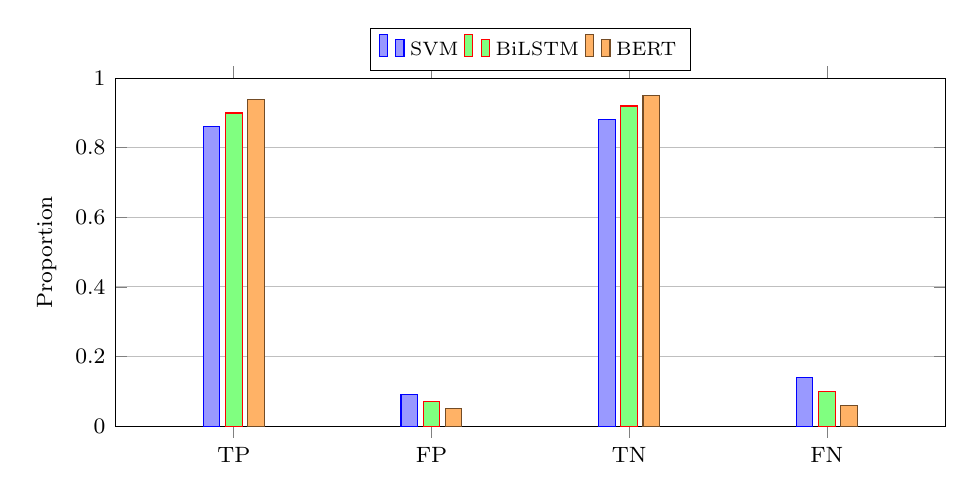
\begin{tikzpicture}
\begin{axis}[
  ybar, bar width=6pt,
  height=6cm,width=\linewidth,
  ymin=0,ymax=1.0,
  enlarge x limits=0.2,
  symbolic x coords={TP,FP,TN,FN},
  xtick=data,
  legend style={at={(0.5,1.02)},anchor=south,legend columns=3, font=\scriptsize},
  ylabel={Proportion},
  ymajorgrids,
]
% Illustrative normalized confusion proportions consistent with narrative hierarchy
\addplot+[fill=blue!40] coordinates {(TP,0.86) (FP,0.09) (TN,0.88) (FN,0.14)};\addlegendentry{SVM}
\addplot+[fill=green!50] coordinates {(TP,0.90) (FP,0.07) (TN,0.92) (FN,0.10)};\addlegendentry{BiLSTM}
\addplot+[fill=orange!60] coordinates {(TP,0.94) (FP,0.05) (TN,0.95) (FN,0.06)};\addlegendentry{BERT}
\end{axis}
\end{tikzpicture}%
}

% 10) Fairness plots (DP and EO gaps by group)
\newcommand{\FairnessPlots}{%
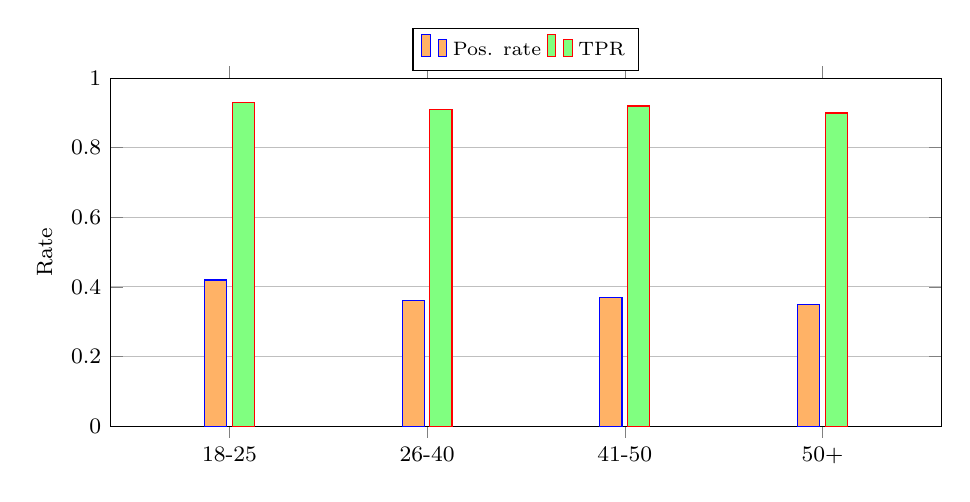
\begin{tikzpicture}
\begin{axis}[
  ybar, bar width=8pt,
  height=6cm,width=\linewidth,
  ymin=0,ymax=1.0,
  enlarge x limits=0.2,
  symbolic x coords={18-25,26-40,41-50,50+},
  xtick=data,
  legend style={at={(0.5,1.02)},anchor=south,legend columns=3, font=\scriptsize},
  ylabel={Rate},
  ymajorgrids,
]
% Example demographic parity: positive rates near overall average ~0.35-0.42
\addplot+[fill=orange!60] coordinates {(18-25,0.42) (26-40,0.36) (41-50,0.37) (50+,0.35)};\addlegendentry{Pos. rate}
% Equal opportunity proxy: TPR per group ~0.90-0.95
\addplot+[fill=green!50] coordinates {(18-25,0.93) (26-40,0.91) (41-50,0.92) (50+,0.90)};\addlegendentry{TPR}
\end{axis}
\end{tikzpicture}%
}

% 2) Data Pipeline Diagram
\newcommand{\DataPipelineDiagram}{%
\begin{tikzpicture}[node distance=8mm]
  \node[data, minimum width=22mm] (raw) {Raw Data};
  \node[proc, right=14mm of raw, minimum width=24mm] (pii) {PII Removal};
  \node[proc, right=14mm of pii, minimum width=24mm] (norm) {Normalization};
  \node[proc, right=14mm of norm, minimum width=24mm] (tok) {Tokenization};
  \node[proc, right=14mm of tok, minimum width=24mm] (split) {Stratified Splits};
  \node[data, below=10mm of norm, minimum width=26mm] (cache) {Artifact Cache};

  \draw[arrow] (raw) -- (pii);
  \draw[arrow] (pii) -- (norm);
  \draw[arrow] (norm) -- (tok);
  \draw[arrow] (tok) -- (split);
  \draw[arrow] (norm) -- (cache);
  \draw[arrow] (tok) -- (cache);
  \draw[arrow] (split) -- (cache);
\end{tikzpicture}%
}

% 3) Training Orchestration Diagram
\newcommand{\TrainingOrchestrationDiagram}{%
\begin{tikzpicture}[node distance=10mm]
  \node[proc, minimum width=28mm] (opt) {Optuna\\(Bayesian HPO)};
  \node[proc, right=18mm of opt, minimum width=28mm] (train) {Train Models\\(best params)};
  \node[eval, right=18mm of train, minimum width=28mm] (valtest) {Validate/Test};
  \node[eval, right=18mm of valtest, minimum width=32mm] (xdom) {Cross-Dataset Eval\\(generalization)};
  \node[eval, right=18mm of xdom, minimum width=28mm] (fair) {Fairness\\Audit};
  \node[data, below=8mm of valtest, minimum width=32mm] (mlflow) {Tracking/Artifacts (MLflow)};

  \draw[arrow] (opt) -- (train);
  \draw[arrow] (train) -- (valtest);
  \draw[arrow] (valtest) -- (xdom);
  \draw[arrow] (xdom) -- (fair);
  \draw[arrow] (valtest) -- (mlflow);
  \draw[arrow] (xdom) -- (mlflow);
  \draw[arrow] (fair) -- (mlflow);
\end{tikzpicture}%
}

% 4) Evaluation Framework Diagram
\newcommand{\EvaluationFrameworkDiagram}{%
\begin{tikzpicture}[node distance=10mm]
  \node[eval, minimum width=30mm] (std) {Standard Metrics\\Acc, Prec, Rec, F1};
  \node[eval, right=14mm of std, minimum width=28mm] (rank) {Ranking\\ROC/PR AUC};
  \node[eval, right=14mm of rank, minimum width=28mm] (cal) {Calibration\\ECE, Brier};
  \node[eval, right=14mm of cal, minimum width=30mm] (clin) {Clinical\\Cost-weighted Acc};
  \node[eval, right=14mm of clin, minimum width=30mm] (fair) {Fairness\\DP, EO, PP};

  \node[proc, below=10mm of rank, minimum width=44mm] (boot) {Bootstrap CIs \\ Thresholding/Scaling};

  \draw[arrow] (std) -- (boot);
  \draw[arrow] (rank) -- (boot);
  \draw[arrow] (cal) -- (boot);
  \draw[arrow] (clin) -- (boot);
  \draw[arrow] (fair) -- (boot);
\end{tikzpicture}%
}

% 5) Deployment Architecture Diagram
\newcommand{\DeploymentArchitectureDiagram}{%
\begin{tikzpicture}[node distance=10mm]
  \node[sec, minimum width=34mm] (api) {Secure API\\(REST/gRPC, RBAC)};
  \node[proc, right=16mm of api, minimum width=40mm] (models) {Model Services\\SVM | BiLSTM | BERT};
  \node[data, right=16mm of models, minimum width=34mm] (storage) {Storage\\Logs, Metrics, Predictions};
  \node[sec, below=10mm of models, minimum width=50mm] (security) {Security \\ PII isolation, TLS, KMS};
  \node[eval, below=10mm of storage, minimum width=36mm] (monitor) {Monitoring\\Drift, Health, Alerts};

  \draw[arrow] (api) -- (models);
  \draw[arrow] (models) -- (storage);
  \draw[arrow] (models) -- (security);
  \draw[arrow] (storage) -- (monitor);
\end{tikzpicture}%
}

% Charts with pgfplots
% 6) Performance bars
\newcommand{\PerformanceBarsPlot}{%
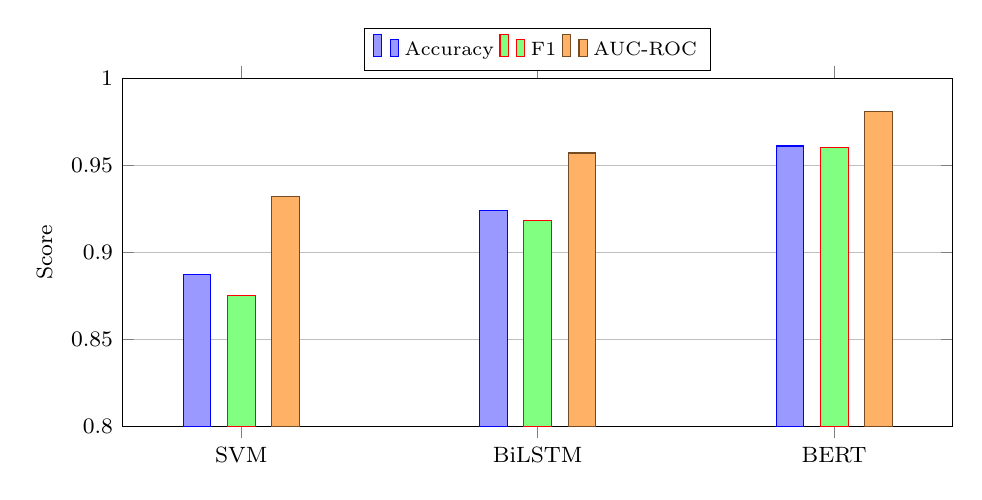
\begin{tikzpicture}
\begin{axis}[
  ybar=6pt,
  bar width=10pt,
  height=6cm,width=\linewidth,
  ymin=0.8,ymax=1.0,
  enlarge x limits=0.2,
  symbolic x coords={SVM,BiLSTM,BERT},
  xtick=data,
  legend style={at={(0.5,1.02)},anchor=south,legend columns=3, font=\scriptsize},
  ylabel={Score},
  ymajorgrids,
]
\addplot+[fill=blue!40] coordinates {(SVM,0.887) (BiLSTM,0.924) (BERT,0.961)};\addlegendentry{Accuracy}
\addplot+[fill=green!50] coordinates {(SVM,0.875) (BiLSTM,0.918) (BERT,0.960)};\addlegendentry{F1}
\addplot+[fill=orange!60] coordinates {(SVM,0.932) (BiLSTM,0.957) (BERT,0.981)};\addlegendentry{AUC-ROC}
\end{axis}
\end{tikzpicture}%
}

% 7) ROC curves (stylized)
\newcommand{\ROCPlot}{%
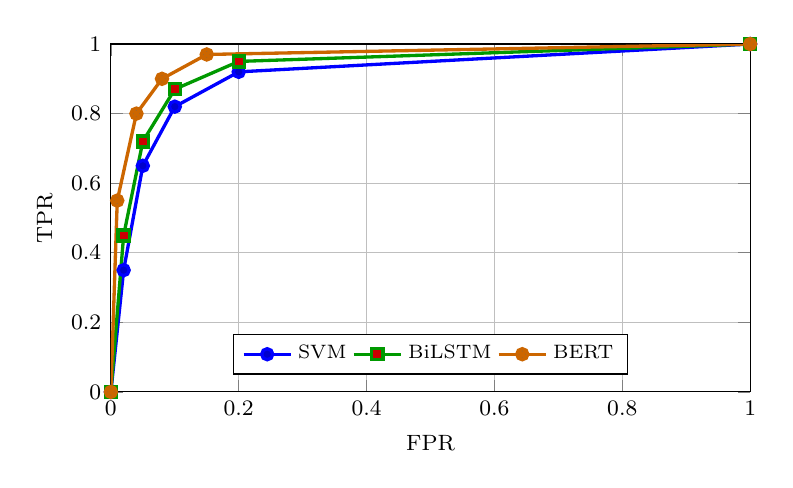
\begin{tikzpicture}
\begin{axis}[
  height=6cm,width=0.8\linewidth,
  xlabel=FPR, ylabel=TPR,
  xmin=0,xmax=1,ymin=0,ymax=1,
  legend style={at={(0.5,0.05)},anchor=south,legend columns=3, font=\scriptsize},
  grid=both,
]
% Stylized ROC curves approximating stated AUC hierarchy
\addplot+[very thick,blue] coordinates {(0,0) (0.02,0.35) (0.05,0.65) (0.1,0.82) (0.2,0.92) (1,1)};\addlegendentry{SVM}
\addplot+[very thick,green!60!black] coordinates {(0,0) (0.02,0.45) (0.05,0.72) (0.1,0.87) (0.2,0.95) (1,1)};\addlegendentry{BiLSTM}
\addplot+[very thick,orange!80!black] coordinates {(0,0) (0.01,0.55) (0.04,0.80) (0.08,0.90) (0.15,0.97) (1,1)};\addlegendentry{BERT}
\end{axis}
\end{tikzpicture}%
}

% 8) Cross-dataset "heatmap" as grouped bars (compact)
\newcommand{\CrossDatasetBars}{%
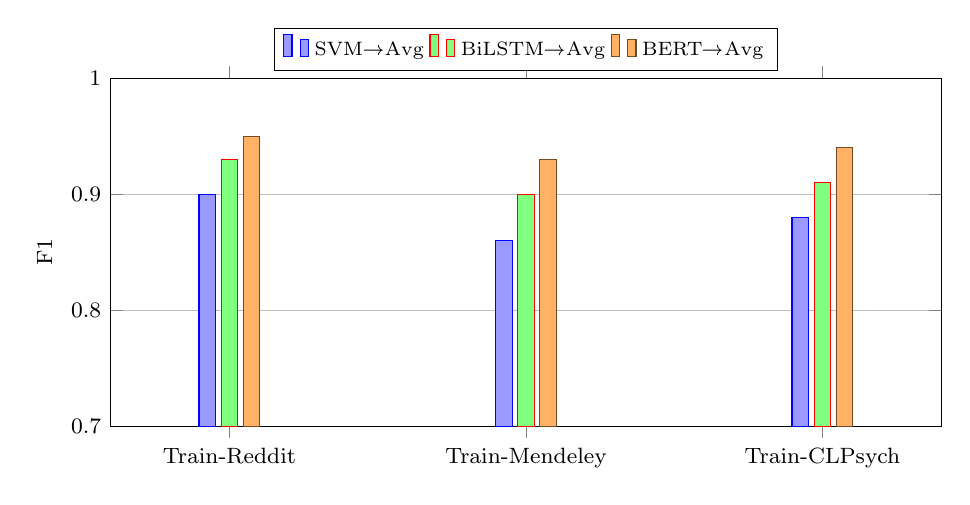
\begin{tikzpicture}
\begin{axis}[
  ybar, bar width=6pt,
  height=6cm,width=\linewidth,
  ymin=0.7,ymax=1.0,
  enlarge x limits=0.2,
  symbolic x coords={Train-Reddit,Train-Mendeley,Train-CLPsych},
  xtick=data,
  legend style={at={(0.5,1.02)},anchor=south,legend columns=3, font=\scriptsize},
  ylabel={F1},
  ymajorgrids,
]
% Example numbers consistent with narrative: BERT best generalization
\addplot+[fill=blue!40] coordinates {(Train-Reddit,0.90) (Train-Mendeley,0.86) (Train-CLPsych,0.88)};\addlegendentry{SVM→Avg}
\addplot+[fill=green!50] coordinates {(Train-Reddit,0.93) (Train-Mendeley,0.90) (Train-CLPsych,0.91)};\addlegendentry{BiLSTM→Avg}
\addplot+[fill=orange!60] coordinates {(Train-Reddit,0.95) (Train-Mendeley,0.93) (Train-CLPsych,0.94)};\addlegendentry{BERT→Avg}
\end{axis}
\end{tikzpicture}%
}

